% Chapter Template

\chapter{Introduction} % Main chapter title

\label{Chapter:1}

Carbon nano-materials are subjected to great interest for research purposes due to their various potential applications in diverse areas that take advantage of the nano-scale properties. Carbon nano-materials are suitable for catalysis, adsorption, carbon capture, energy and hydrogen storage, drug delivery, bio-sensing, and cancer detection. Some matchless properties that allow carbon nano-materials to be utilized within multiple functionalities include high porosity, distinguished structures, uniform morphologies, high stability, high magnetic properties, and high conductivity. \cite{McCreery2008, Geim2011, Zhu2010, Katsnelson2008, Li2008, Geim2007, Geim2009, Siddiqui2019}

This document bestows a thesis project to perform research to engineer a polymer solution to achieve mass scale manufacturing of high conductive carbon nano-wires with a reduced diameter in an inexpensive, continuous, simple and reproducible manner. The research intends to involve several manufacturing processes such as near field electrospinning, photo-polymerization, pyrolization, and carbonization, as they have shown to be promising methods for the fabrication of carbon nano-materials. \cite{Cardenas2017} See Figure \ref{fig:fabricationFlowChart}. A number of processes have been developed for specific purposes of polymeric nano-fibres, some include surface deposition, composites, and chemical adjustments. Polymeric nano-fibers must be also pyrolyzed to generate carbon nano-wires with conductive capabilities \cite{Madou2011} for electrochemical sensing and energy storage purposes.

\begin{figure}[th]
\centering
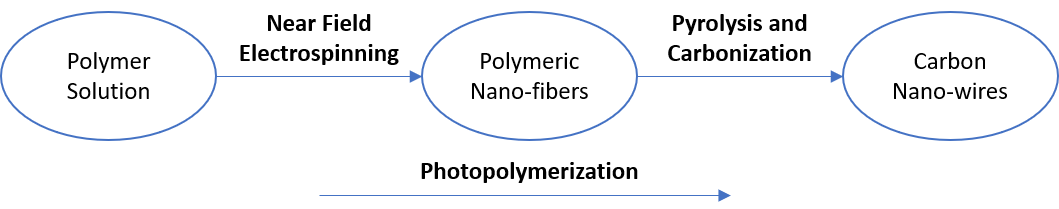
\includegraphics[width=1.0\textwidth]{./Figures/FabricationProcess.png}
\decoRule
\caption[Fabrication Process of Carbon Nano-wires]{Fabrication process and characterization techniques of conductive carbon nano-wires to achieve through the dissertation.}
\label{fig:fabricationFlowChart}
\end{figure}

Nanotechnology has led to the study of different polymer patterning techniques to integrate carbon nano-wires structures. One technique is known as far-field electrospinning (FFES), a process in which electrified jets of polymer solution are dispensed to synthesize nano-fibres which are then pyrolyzed at high temperatures. One sub-technique derived from electrospinning is near-field electromechanical spinning or NFEMS. Unlike FFES, NFEMS has proved to deliver high control in patterning polymeric nano-fibres. \cite{Cardenas2017}

The proposal is to continue the previous work done in regards to the synthesis of carbon nano-wires. Previous work includes the fabrication of suspended carbon nano-wires by two methods: electro-mechanical spinning and multiple-photon polymerization with a photoresist. \cite{Cardenas2017, Flores2017} This work is intended to focus on electro-mechanical spinning processes only, to bring off polymer solutions that can be electrospun by NFEMS, photo-polymerized and pyrolyzed into conducting carbon nano-wires. The polymer solutions described by Cárdenas and Flores \cite{Flores2017, Cardenas2017} are to be amended to achieve the goal mentioned in the previous statement.

Traditional near-field electrospinning or NFES allows large scale manufacturability combined with spatial control of material deposition. \cite{Madou2011} However, the reported efforts required the use of electric fields in excess of 200 kV/m for continuous operation, resulting in limited control for nano-fiber patterning in traditional NFES processes. Madou et al. \cite{Madou2011} conclude that the current state-of-the-art synthesis processes for polymer nano-fibers lack to yield precise, inexpensive, fast, and continuous manufacturing properties.

%----------------------------------------------------------------------------------------
%	SECTION 1
%----------------------------------------------------------------------------------------
\section{Carbon Nanowires Research Developments in Terms of Published Papers, Synthesis and Fabrication}

% \cite{Rauti2019}

Nanotechnology ability to control and piece together materials at the nano-scale has enabled the development of various carbon nano-materials and carbon nano-structures, such as nano-dots, nano-fibres, nano-tubes and nano-wires. \cite{Posthuma-Trumpie2012, Zhang2009, DeVolder2011, Cao2011} This chapter bestows on the applications at the micro-scale and nano-scale levels, as well as the current research of carbon-based nano-materials (CBNs).

\subsection{Carbon and carbon-based nanomaterials}

\begin{figure}[th]
\centering

\includegraphics[scale=0.40]{./Figures/CBNfingerprint.png}
\decoRule
\caption[Fingerprint of Carbon-based Nano-materials]{Molecular to mesoscale structural features of synthetic polymers influence the emergence of specific microstructural features in polymer-derived carbon materials after pyrolysis.}
\label{fig:CBNfingerprint}
\end{figure}

Carbon is a versatile element capable to form a number of bonds with other elements or with itself. Cabon-based nano-materials (CBNs) exist in diverse forms, depending on the precise values of each degree of freedom that specify the material proclivity at multiple scales. Hybridization, crystallization, percolation, anisotropy, porosity, impurities and imperfections are some of the relevant features that determine the CBN set of properties. The combination of these features at the micro- and meso-scale burst a variety of macro-scale properties that comprise the CBN fingerprint (\ref{fig:CBNfingerprint}). The interminable collection of possible CBN fingerprints range from soft, conductive lubricants to very hard, low conductivity solids; and from black colour, bulks to transparent, disordered thin films. \cite{McCreery2008} Figures \ref{fig:carbonAllotropes} and \ref{fig:carbonAllotropesDiagram} shows the existence of different types of allotrope as carbon orbitals have the ability to hybridize in sp1, sp2 and sp3 configurations, assembling different types of allotropes.

\begin{figure}[th]
\centering

\includegraphics[scale=0.30]{./Figures/carbonAllotropes.png}
\decoRule
\caption[Carbon sp-hybrid Nano-materials]{Three carbon allotropes (diamond, carbyne and graphene) are the building blocks of additional deriving carbon types such as fullerenes, porous carbon and glass-like carbon.}
\label{fig:carbonAllotropes}
\end{figure}

\begin{figure}[th]
\centering
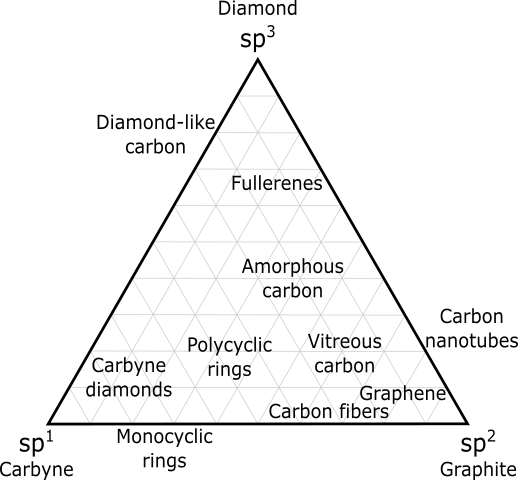
\includegraphics[scale=0.65]{./Figures/carbonAllotropesHybridization.png}
\decoRule
\caption[Ternary Diagram of Carbon Allotropes based on sp Content]{Ternary phase diagram of amorphous carbon regions based on hybridization degree. Adapted from \cite{Heersche2007, Heimann1997, Belenkov2003, Fedel2013, Razeghi2019, AlstrupJensen2015, Vajtai2013}.}
\label{fig:carbonAllotropesDiagram}
\end{figure}

In terms of porosity, CBNs exhibit different properties according to the degree of 'open' and 'closed' pores. A 'closed pore' is a void or empty space in solid materials where a discontinuity is present within the array of atoms and molecules. On the other hand, an 'open pore' refers to a void which is connected to the outer surface of the solid, in other words a 'open pore' is a 'closed pore' with an opening to the external surface. \cite{Marsh1989} Figure \ref{fig:carbonAllotropesPorosityNOrder} shows a classification of carbon allotropes according to their porous content.

\begin{figure}[th]
\centering
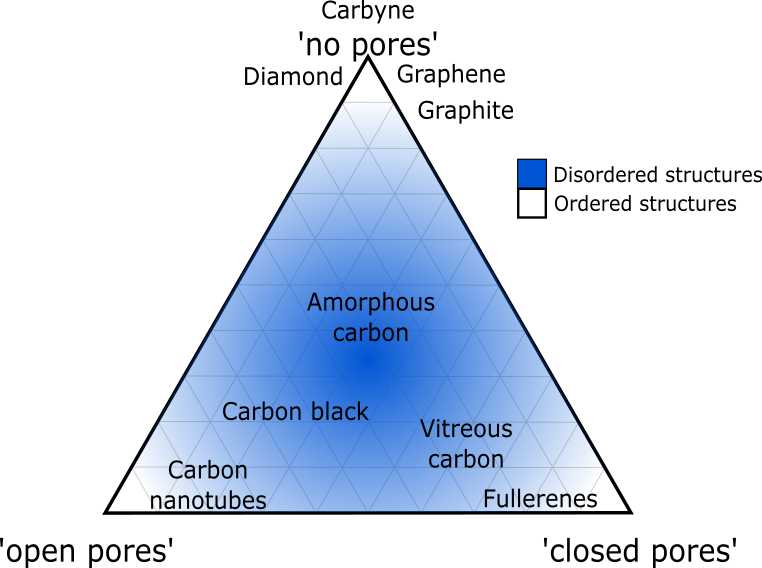
\includegraphics[scale=0.65]{./Figures/carbonAllotropesPorosityNOrder.png}
\decoRule
\caption[Ternary Diagram of Carbon Allotropes based on Porosity and Structural Order]{Ternary phase diagram of amorphous carbon regions based on structure order and porosity. Regions are colored by the degree of crystalline order within the carbon structure. White represents highly ordered structures, whereas white represents disordered structures. \cite{Marsh1989, Hugh1994}}
\label{fig:carbonAllotropesPorosityNOrder}
\end{figure}

Thermal conductivity and electrical conductivity decrease with increasing porosity due to the reduced amount of material to conduct electrons and energy. Furthermore, porosity negatively affects the mechanical properties like strength and elastic modulus as it reduces the volume in which stresses are distributed. Moreover, stresses are concentrated at the pores which makes the material prone to mechanical failure. \cite{Marsh1989, Hugh1994}

Due to the versatility and variety of CBNs, CBNs have been fabricated and implemented for various purposes. \cite{Geim2011, Katsnelson2008, Li2008, Geim2007, Geim2009, Siddiqui2019}. For instance, field effect transistors (FET) have been studied by Novoselov \cite{Novoselov2004} and Heersche et. al. \cite{Heersche2007}. Carbon FET devices have reported field-effect mobility one order of magnitude higher than that of silicon FETs. Other literature suggests CBNs to be favorable to detect a variety of gases and bio-molecules. \cite{Schedin2007, Ohno2009} As molecules are absorbed by the CBN, the carrier density and electrical resistivity of the carbon material changes. Moreover, CBNs have showed good performance in applications in energy (prevent wastage of energy), water (purification) and diagnostics (lab-on-chip systems and nano-sensors). \cite{Cao2011, Khanna2016} As mentioned above, the morphology of CBNs has an impact on the electrochemical and mechanical properties. \cite{Marsh1989, Hugh1994, Guo2018} In this regard, carbon nano-structures, such as nano-wires \cite{Kundu2019, Bencheikh2019, Bencheikh2019}, have been fabricated to achieve improved electrochemical characteristics.

\subsection{Carbon nanowires}

As depicted in Figure \ref{fig:carbonAllotropesDiagram}, carbon nano-fibers (CNFs) have been classified as linear, sp2-based structures. \cite{Heersche2007, Heimann1997, Belenkov2003, Fedel2013, Razeghi2019, AlstrupJensen2015, Vajtai2013} Nano-fibers own good electrical, optical and mechanical characteristics, however those properties are highly dependent on the morphology of the fibers. \cite{Dresselhaus2007} The material properties of 1D nano-structures depend on fiber diameter, porosity, crystallization degree and crystallization orientation. Consequently, the fabrication parameters and environment conditions have an impact on the reproducibility of high quality fibers. \cite{Dresselhaus2007}

Carbon nano-fibers (CNF) have diameters of several micrometers and are different from carbon nano-tubes (CNT). \cite{Weil1992, Huang2009, chung2012carbon, Subramoney1997, Dresselhaus2000} 

\subsection{Nanowires synthesis}

%%%
Numerous methods to prepare nanowires, which include template-assisted synthesis [30], vapor–liquid-solid (VLS) [31], electrodeposition [32], electrospinning [33], hydrothermal [34], also hierarchical arrangement techniques [35–37] to organize the nanowires have been studies in the last ten years. Nanowires based on organic, inorganic or hybrid materials have been applied in order to get single or composites nanomaterials for innumerous purposes, such as chemical and biochemical sensing devices, thermoelectric, optical, magnetic and electrical application. In this section, we are focusing on the synthesis of conducting polymer and composites to develop materials in nanowires architectures.

\subsubsection{Synthesis of conducting polymer nanowires}



\subsection{\emph{conclude that NFES is the way to go}}




%----------------------------------------------------------------------------------------
%	SECTION 2
%----------------------------------------------------------------------------------------
\section{Problem definition and motivation}

%Qué metodos se han utilizado? (SU-8)
%Porqué se quiere fabricar las fibras de carbono
%Para qué aplicaciones se han usado
%Porqué es importante la conductividad
%Porqué es importante que sea puro carbono

Carbon nanowires have been fabricated with a photoresist by multiple-photon polymerization techniques. However little is known about polymers that can produce conductive carbon nano-wires after pyrolysis, as it is generally believed that most polymers do not form significant amounts of graphitic carbon when carbonized.
%The lack of research relays on the fact that in the past years, it was assumed that most polymers are non-graphitic through pyrolysis \cite{Franklin1951}.
In the past years, photopolymerization processes have been applied to the fabrication of nano-structures with the use of an epoxy based photoresist. \cite{Boer2014} Photopolymerization techniques deliver patterning resolutions with nano-scale tolerances through two-photon lithography for the production of highly detailed structures \cite{Hribar2014}.

On the other hand, electrospinning has been acknowledged as a process with promising results at nano-structure fabrication \cite{Boer2014}, yet there is little research regarding the implementation of electrospinning for the fabrication of carbon nano-wires. Electrospinning has the potential to be a more straightforward process for the design and fabrication of nano-structures, as it can achieve mass scale manufacturing in a continuous, simple and reproducible manner. Cardenas \cite{Cardenas2017} showed that electrospinning can be implemented with ease for carbon nano-wire synthesis. Mechano-electrospinning, a new variant of electrospinning shows promising results in the production of ordered carbon nano-wires. As stated in \cite{Cardenas2017}, mechano-electrospinning is an early technology invention and brings new challenges, such as the reproducibility of carbon nano-wire production. Furthermore, the study of a new fabrication process to produce carbon nanowires that involves mechano-electrospinning will enable spatial control of the structures' patterning.

Since electrospinning seems to be a better alternative for carbon nano-wire fabrication processes; and for that purpose of its implementation, it is required to develop polymer solutions that can be mechano-electrospun, photopolymerized and pyrolyzed into conducting carbon nano-wires. Carbon nano-materials have been subjected to research due to their various potential applications in diverse areas that take advantage of the nano-scale properties. \cite{Siddiqui2019} Carbon nano-materials are suitable for the catalysis, adsorption, carbon capture, energy and hydrogen storage, drug delivery, bio-sensing and cancer detection. \cite{Siddiqui2019} However most applications are not currently feasible due to the lack of a continuous, simple and reproducible fabrication method with inexpensive processes. With the newly designed polymer solution, it would be possible to produce carbon nano-wires in large quantities, and therefore more applications will become feasible. On the other hand, the new technique will overcome some limitations of other methods such as lithography currently has. For instance, patterns created by lithography processes cannot be originated, only replicated, all constituent points of the pattern can only be addressed at the same time, and the process requires the pattern to be encoded into a mask. \cite{Landis2011}

%----------------------------------------------------------------------------------------
%	SECTION 3
%----------------------------------------------------------------------------------------
\section{Hypothesis}

The rheological properties of polymer solutions along with synthesis parameters (stage velocity, voltage, dispense rate) can be amended through rheological analyses to obtain a low voltage electrospun-able, photopolymerizable and graphitizable fibers for the fabrication conductive of carbon nano-wires with specified dimensions (diameter and length). The rheological properties of polymer solutions along with synthesis parameters are to be amended by replacing the PEO (Poly(ethylene) oxide) component within the existing polymer solutions described in Flores \cite{Flores2017} and Cardenas \cite{Cardenas2017} work. PEO is to be replaced as its only purpose is to allow the electrospinning process to take place, but no benefit is obtained from it after pyrolysis.

%----------------------------------------------------------------------------------------
%	SECTION 4
%----------------------------------------------------------------------------------------
\section{Research Questions}

\begin{itemize}
	\item{
	Is there any evidence of conductive carbon nano-wire fabrication though electrospun-able and pyrozable polymer solutions?
	}
	\item{
	What are the process parameters to consider/control for the fabrication processes of carbon nano-wires? 
	}
	\item{
	What rheological properties are to be controlled/tested to deliver an electrospun-able and pyrozable polymer solution?	
	}
	\item{
	Are there any efforts employed to the design of polymer solutions that can be electrospun, photopolymerized, and pyrolyzed into conducting carbon nanowires?
	}
	\item{
	What are the optimal fabrication parameters for the synthesis of carbon nano-wires through near-field electromechanical spinning?	
	}
	\item{
	What materials can be used to ease the electrospinning process and favor the carbon nano-wire properties after pyrolysis? 
	}
\end{itemize}

%----------------------------------------------------------------------------------------
%	SECTION 5
%----------------------------------------------------------------------------------------
\section{Objectives}

\subsection{General objective}
Study the practice and feasibility of a new fabrication process to achieve mass scale manufacturing of carbon nano-wires in an inexpensive, continuous, simple and reproducible manner; by the integration of mechano-electrospinning technique.

\subsection{Specific objectives}

\begin{itemize}
	\item{
	Design polymer solutions that can be electrospun by NFES, photopolymerized, and then pyrolyzed.
    }
    \item{
    Through rheological analyses, determine if polymer solutions can be easily employed for conducting carbon nano-wire synthesis.
    }
    \item{
    Determine and control the polymer solution rheological properties along with the process parameters of carbon nano-wire synthesis.
    }
    \item{
    Discover a PEO-similar material to allow the electrospinning process as well as input favourable properties to the carbon nano-wire yield.
    }
\end{itemize}

%----------------------------------------------------------------------------------------
%	SECTION 6
%----------------------------------------------------------------------------------------
\section{Dissertation Outline}


